\chapter{Esperimenti}
\label{cap:Esperimenti}
Gli esperimenti sono stati condotti seguendo i settaggi originali di AMEGO. Di seguito vengono riportate le principali impostazioni utilizzate.

Per l'identificazione delle interazioni mano-oggetto a livello di frame è stato utilizzato l'\emph{Hand-Object Interaction detector} \cite{shan2020understandinghumanhandscontact}.  
Le feature visive degli oggetti sono state estratte tramite il modello pre-addestrato \emph{DINO-v2} \cite{oquab2024dinov2learningrobustvisual}, con ridimensionamento in fase di valutazione sulla versione \emph{ViT-L}.  

Il tracciamento degli oggetti durante le interazioni è stato gestito tramite l'EgoSTARK tracker \cite{tang2023egotrackslongtermegocentricvisual}, con i seguenti parametri:

\begin{itemize}
    \item $\theta = 0.6$: soglia di similarità per l'associazione dei bounding box.
    \item $w_s = 30$: finestra temporale di frame utilizzata per garantire la coerenza spaziale.
    \item $s_o = 20$: numero minimo di bounding box consecutivi con forte sovrapposizione spaziale richiesto per definire un tracklet.
    \item $e_o = 20$: numero massimo di frame consecutivi senza rilevazioni associate prima di considerare un tracklet terminato, purché la mano rimanga visibile.
\end{itemize}

Come estrattore di feature per le location è stato utilizzato \emph{SWAG} \cite{singh2022revisitingweaklysupervisedpretraining}.

L'\emph{optical flow} è stato stimato tramite il modello Flowformer \cite{huang2022flowformertransformerarchitectureoptical}, adottando i seguenti parametri:

\begin{itemize}
    \item $\theta = 2000$: soglia applicata alla norma L2 dell'optical flow.
    \item $s_l = 5$: numero minimo di frame consecutivi richiesti per considerare attivo un \emph{Location segment} $l_j$.
    \item $e_l = 5$: numero massimo di frame consecutivi per cui si tollera che 
    la norma dell'optical flow superi la soglia massima oppure che non vengano 
    rilevate mani; se tale limite viene superato, il segmento $l_j$ viene terminato.
    \item $\tau = 0.5$: soglia minima di similarità richiesta per assegnare un segmento $l_j$ a una location già esistente.
\end{itemize}

Di seguito vengono riportate le fasi principali di sperimentazione.

Il notebook e altre risorse che forniscono ulteriori dettagli sui lavori svolti sono disponibili nella repository GitHub del progetto: 
\begin{center}
    \footnotesize
    \href{https://github.com/Kespers/Egocentric-Videos-Understanding-with-Active-Memory}{https://github.com/Kespers/Egocentric-Videos-Understanding-with-Active-Memory}
\end{center}

\section{Setup ambiente}

Per poter eseguire il progetto AMEGO in tutte le sue componenti, gli autori consigliano due ambienti \texttt{conda} separati, ciascuno con versioni di \texttt{python} e dipendenze differenti. In particolare:
\begin{itemize}
    \item l'ambiente \texttt{amego}, basato su \texttt{python 3.9}, necessario per lanciare gli script nativi del framework;
    \item l'ambiente \texttt{handobj}, basato su \texttt{python 3.8}, per eseguire lo script di \emph{hand-object detection};
\end{itemize}

Il carico computazionale richiesto da questi task necessita dell'utilizzo di hardware apposito. Per questo motivo non è stato possibile condurre gli esperimenti su una macchina personale, ma si è fatto ricorso alle risorse messe a disposizione dal Dipartimento di Matematica e Informatica dell'Università di Catania.  

In un contesto di questo tipo, è fondamentale garantire isolamento e riproducibilità degli ambienti di lavoro. Per questo motivo si è scelto di adottare un approccio basato su \emph{Docker}, integrando i due ambienti \texttt{conda} in un unico container.

Il \texttt{Dockerfile} è stato strutturato partendo da \texttt{Ubuntu} come immagine di base. Su questa base è stato installato \emph{Miniconda}, impiegato come gestore principale degli ambienti virtuali, permettendo così di mantenere all'interno dello stesso container due ambienti \texttt{conda} separati.  
È stata inoltre definita una directory di lavoro centrale, \texttt{/workspace/amego}, contenente il codice del progetto e gli script di setup. All'interno del container, nella directory \texttt{/workspace/ENIGMA-51}, è stata montata la partizione \texttt{/dataset/ENIGMA-51} del server, contenente l'intero contenuto del dataset, inclusi frame e annotazioni.

La build iniziale è stata tentata su una macchina equipaggiata con GPU \textbf{Tesla K80}. Tuttavia, la scheda video risulta troppo obsoleta e non supporta le versioni più recenti delle librerie necessarie.

Per l'esecuzione degli esperimenti è stato utilizzato un server con risorse più recenti, di seguito sono riportate le caratteristiche principali:

\begin{table}[H]
    \centering
    \begin{tabular}{ll}
        \hline
        \textbf{Componente} & \textbf{Specifiche principali} \\
        \hline
        CPU & Intel(R) Xeon(R) Silver 4210 @ 2.20GHz \\
        GPUs & 3x Tesla V100S (32GB), 1x Tesla V100 (16GB) \\
        \hline
    \end{tabular}
    \caption{Specifiche hardware utilizzato.}
\end{table}


Su questa infrastruttura, la build del container è andata a buon fine ed è stato possibile eseguire correttamente le procedure necessarie ad AMEGO.  

In particolare, le operazioni principali sono state le seguenti:
\begin{enumerate}
    \item \textbf{Download del video di test:} è stato scaricato il video \texttt{P01\_01} del dataset EPIC-KITCHENS \cite{Damen2021PAMI} utilizzando gli script ufficiali forniti dai creatori del dataset \cite{epic_download_scripts}.
    \item \textbf{Estrazione dei frame:} il video è stato convertito in sequenze di frame.
    \item \textbf{Hand-object detection:} generazione dei bounding box relativi alle hand-object-detections per ciascun frame.
    \item \textbf{Estrazione Optical flow}
    \item \textbf{AMEGO HOI / Location Segments:} creazione delle componenti di memoria di AMEGO
    \item \textbf{Query:} esecuzione delle query AMB
\end{enumerate}

Dopo aver verificato il corretto funzionamento dell'intera pipeline, è stato quindi possibile passare agli esperimenti principali su ENIGMA-51.

\section{AMB su ENIGMA-51}

Analogamente a quanto fatto per EPIC-KITCHENS, sono stati eseguiti gli script di AMEGO per estrarre le componenti indispensabili al funzionamento del metodo. La differenza è l'uso della partizione montata che ha agevolato la parte di estrazione frame in quanto erano già forniti.

\subsection*{Elaborazione files}
Un primo lavoro ha riguardato la strutturazione delle cartelle. Data la struttura dei loader usati da AMEGO, è suggerita la seguente organizzazione:
\begin{center}
    \begin{verbatim}
        <video_id>/
            rgb_frames/
                frame_0000000000.jpg
                frame_0000000001.jpg
                ...
            flowformer/
                flow_0000000000.pth
                flow_0000000001.pth
                ...
            hand-objects/
                <video_id>.pkl
    \end{verbatim}    
\end{center}

In ENIGMA i frame dei video sono forniti in un'unica cartella con il formato:
\begin{center}
\texttt{\textbf{<VIDEO-ID>}\_\textbf{<FRAME-ID>}.png}    
\end{center}
Inoltre la risoluzione fornita è (\texttt{2272 $\times$ 1278}), mentre AMEGO si aspetta (\texttt{456 $\times$ 256}). A tal proposito è stato sviluppato uno script Python che ristruttura e ridimensiona correttamente tutti i file.

Con queste basi è stato possibile creare i benchmark su cui testare la memoria. Come anticipato in precedenza, l'attenzione è stata posta sulle query di tipo \textbf{concurrency}, in particolare sulla query Q5. Inizialmente si era considerata anche la Q6, ma per motivi che saranno approfonditi in seguito, non è stato possibile includerla negli esperimenti.

Per la costruzione del benchmark su ENIGMA-51, le annotazioni disponibili sono state rielaborate al fine di generare i file JSON richiesti da \emph{AMEGO} per l'esecuzione delle query.

\subsection*{Q5: What did I use with [VQ]?}

La query Q5 valuta la capacità del modello di riconoscere oggetti utilizzati simultaneamente con un altro oggetto.

Il set di domande è strutturato come segue:
\begin{itemize}
    \item \textbf{id:} Identificativo univoco della domanda
    \item \textbf{video\_id:} Identificativo del video di riferimento
    \item \textbf{question:} Testo della domanda
    \item \textbf{question\_image:} Crop del frame contenente l'oggetto VQ
    \item \textbf{answers:} Cinque possibili risposte
    \item \textbf{correct:} ID della risposta corretta
\end{itemize}

\subsubsection*{Creazione risposte}
Per generare le query, si è proceduto selezionando le annotazioni in cui erano presenti almeno due interazioni \emph{hand-object} simultanee tra oggetti di diversa categoria. Il primo oggetto dell'interazione è stato utilizzato come \texttt{question\_image}, mentre le risposte sono state composte includendo:

\begin{itemize}
    \item \textbf{RISPOSTA CORRETTA}: secondo oggetto dell'interazione;
    \item \textbf{RISPOSTE ERRATE}: vengono utilizzate le \textbf{classi} degli altri oggetti presenti nella scena come riferimento per selezionare lo stesso oggetto in altri punti dello \emph{stesso} video (aspetto importante, poiché non è garantito che in video diversi compaiano gli stessi oggetti). Se gli oggetti generati nelle risposte sono meno di quattro, il set viene completato con classi scelte casualmente.
\end{itemize}

\subsubsection*{Tre versioni per ogni oggetto}
Per ogni classe sono state selezionate tre patch differenti, temporalmente distinte di almeno 0,5 secondi l'una dall'altra, per mostrare diverse pose e ridurre gli effetti di occlusione tipici della visione egocentrica, ad esempio dovuti alle mani del soggetto o ad altri oggetti.

\begin{figure}[ht]
    \centering
    \begin{subfigure}[b]{0.32\linewidth}
        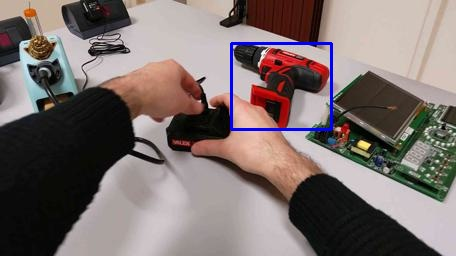
\includegraphics[width=\linewidth]{Images/enigma_am_IMGVER1.jpg}
        \caption{}
        \label{fig:imgver1}
    \end{subfigure}
    \hfill
    \begin{subfigure}[b]{0.32\linewidth}
        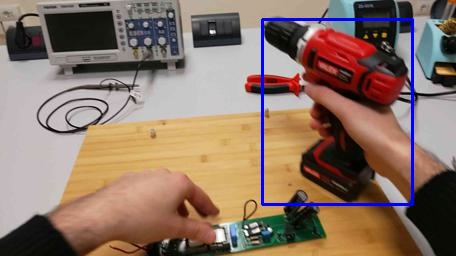
\includegraphics[width=\linewidth]{Images/enigma_am_IMGVER2.jpg}
        \caption{}
        \label{fig:imgver2}
    \end{subfigure}
    \hfill
    \begin{subfigure}[b]{0.32\linewidth}
        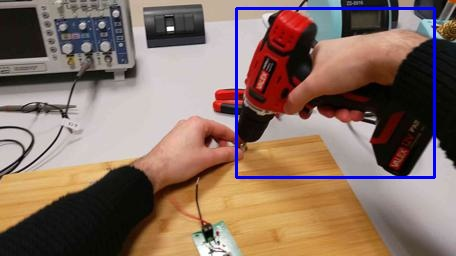
\includegraphics[width=\linewidth]{Images/enigma_am_IMGVER3.jpg}
        \caption{}
        \label{fig:imgver3}
    \end{subfigure}
    \caption{Versioni create per l'oggetto cacciavite}
    \label{fig:enigma_am_screwdrivers}
\end{figure}

\subsubsection*{Conversione formato bounding box}
Infine, è stata effettuata una conversione del formato dei bounding box: le annotazioni originali fornivano i box come 
\begin{center}
\([x_\text{min}, y_\text{min}, \text{width}, \text{height}]\)
\end{center}

mentre AMEGO richiede:
\begin{center}
\([x_\text{min}, y_\text{min}, x_\text{max}, y_\text{max}]\)
\end{center}

Dopo questa operazione è stato quindi generato il file json per fare partire la query.


\subsubsection*{Esempio}
\begin{figure}[h!]
    \centering
    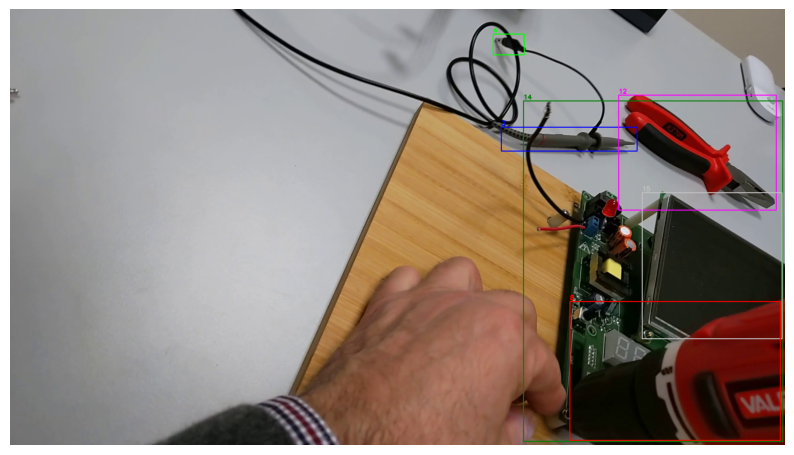
\includegraphics[width=1\linewidth]{Images/q5_ex_annotations.png}
    \caption{
        Frame 46\_6043.jpg annotato con i seguenti oggetti e relativi indici/colori: 
        0: power\_supply (grigio), 
        4: oscilloscope\_ground\_clip (verde), 
        12: pliers (magenta), 
        14: low\_voltage\_board (verde scuro), 
        3: oscilloscope\_probe\_tip (rosso), 
        15: low\_voltage\_board\_screen (argento).
    }
    \label{fig:q5ex}

\end{figure}

Come si nota dalla Fig.~\ref{fig:q5ex}, l'interazione simultanea avviene tra \textbf{low voltage board} e \textbf{electric screwdriver}. Questi due elementi saranno quindi trattati rispettivamente come \textbf{VQ} e \textbf{CORRECT ANSWER}. In questo caso particolare, con gli altri oggetti presenti nella scena, riusciamo ad arrivare a 4 elementi.

Quindi, la query avrà la seguente forma:

\begin{verbatim}
{
 "id": "Q5_000000",
 "video_id": "46",
 "question": "What did I use with [VQ]?",
 "question_image": {
     "low_voltage_board": <INFO>
 },
 "answers": {
     "1": {"oscilloscope_ground_clip": <INFO>},
     "2": {"electric_screwdriver": <INFO>},
     "3": {"oscilloscope_probe_tip": <INFO>},
     "4": {"pliers": <INFO>},
     "5": {"low_voltage_board_screen": <INFO>}
 },
 "correct": 2
}
\end{verbatim}

All'interno di ogni oggetto (\texttt{<INFO>}) troviamo le informazioni riguardo le 3 patch visuali. In particolare:
\begin{verbatim}
{
    "OBJECT": [
        [<frame_1>,[x0, y0, x1, y1]]
        [<frame_2>,[x0, y0, x1, y1]]
        [<frame_3>,[x0, y0, x1, y1]]
    ]
}
\end{verbatim}


\subsection*{Q6: Where did I use [VQ]?}
La query Q6 avrebbe testato la capacità del modello di identificare le location in cui è stato utilizzato un oggetto.

Tuttavia, le annotazioni di ENIGMA non fornivano informazioni sufficienti sulla posizione dei soggetti nei frame. In un primo momento si era ipotizzato di estrarre parole chiave dai file testuali delle procedure per inferire possibili location; tuttavia, il numero limitato di ambienti estraibili e la mancanza di corrispondenza con i frame annotati hanno reso questa sperimentazione poco praticabile.  

In alternativa, sfruttando le location estratte da \emph{AMEGO}, sono stati individuati \textbf{10} cluster.

\begin{figure}[ht]
    \centering
    \begin{minipage}{0.32\textwidth}
        \centering
        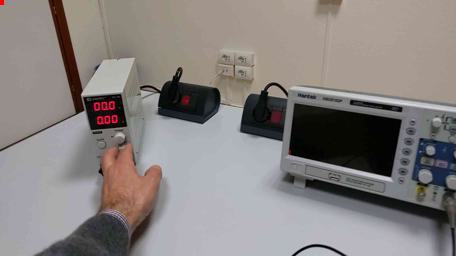
\includegraphics[width=\linewidth]{Images/amego_loc0.jpg}
        \caption*{\texttt{cluster=0}}
    \end{minipage}
    \begin{minipage}{0.32\textwidth}
        \centering
        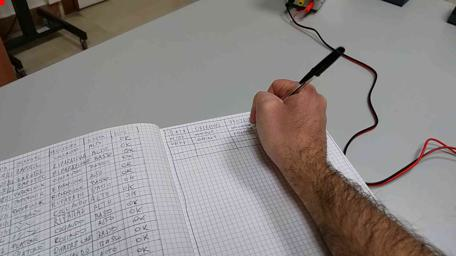
\includegraphics[width=\linewidth]{Images/amego_loc1.jpg}
        \caption*{\texttt{cluster=5}}
    \end{minipage}
    \begin{minipage}{0.32\textwidth}
        \centering
        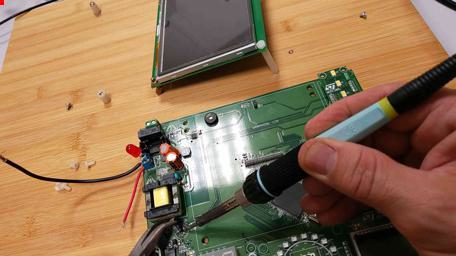
\includegraphics[width=\linewidth]{Images/amego_loc2.jpg}
        \caption*{\texttt{cluster=3}}
    \end{minipage}
    \caption{Esempi di location individuate da \emph{AMEGO} con i relativi cluster assegnati.}
    \label{fig:amego_locations}
\end{figure}

Un'analisi manuale dei cluster ha mostrato che le possibili location corrispondono a: scrivania, area strumenti da tavolo, zona riparazione, consultazione, zona quaderno e quadro elettrico.  

Sono però emerse alcune criticità: le location risultano spesso mescolate, con cluster che vengono considerati unici ma che in realtà dovrebbero essere suddivisi; inoltre, le riprese sono molto statiche e, per questa ragione, anche con annotazioni più accurate non si otterrebbero location realmente significative.  

Alla luce di queste considerazioni, per questo tipo di query sarebbe più opportuno utilizzare un dataset industriale differente, caratterizzato da una maggiore varietà di postazioni, da cui costruire un benchmark più affidabile. Per tali motivi, il lavoro si è concentrato esclusivamente sulla query Q5.

\section{Analisi}

\subsection*{Tempi di esecuzione}

Di seguito sono riportati i tempi approssimativi di esecuzione dei vari script, eseguiti in sequenza sul test-set ENIGMA-51.
Si nota come la fase più dispendiosa sia l'estrazione delle hand-object detections e dell'optical flow, che richiedono circa 30 ore di calcolo.

\begin{table}[ht]
    \centering
    \caption{Tempi di elaborazione dei vari script}
    \begin{tabular}{|l|c|}
        \hline
        \textbf{Script} & \textbf{Tempo} \\
        \hline
        HOI & $\approx$ 30h \\
        OPTICAL FLOW & $\approx$ 30h \\
        AMEGO HOI TRACKLETS & $\approx$ 26h \\
        LOCATION SEGMENTS & $\approx$ 8h \\
        Q5 QUERY & $\approx$ 30min \\
        \hline
    \end{tabular}
    \label{tab:tempi}
\end{table}

\subsection*{Visualizzazione cluster}
Come anticipato nella discussione relativa alla query Q6, è stato sviluppato uno script che consente di visualizzare in modo approfondito la memoria generata. Lo script crea due cartelle principali: \textbf{HOI\_FRAME} e \textbf{LS\_FRAME}.  

All'interno di ciascuna cartella vengono generate sottocartelle corrispondenti ai cluster individuati, contenenti i relativi frame.\\
Nel caso di \texttt{HOI\_FRAME}, per ogni immagine viene inoltre disegnato il bounding box corrispondente.

\subsection*{Visualizzazione video}

Per avere una visione d'insieme della memoria creata da AMEGO, è stato realizzato uno script che, dato un video, raggruppa i vari HOI tracklets trovati e li sovrappone con i rispettivi bounding.
Come mostrato in Fig.~\ref{fig:amego_video}, nella parte superiore del video sono visualizzate informazioni generali sul tipo di video e sul frame corrente. Al centro scorrono i frame con disegnati i bounding box dei vari HOI, ciascuno caratterizzato da un colore assegnato univocamente a ogni cluster.

\begin{figure}[ht]
    \centering
    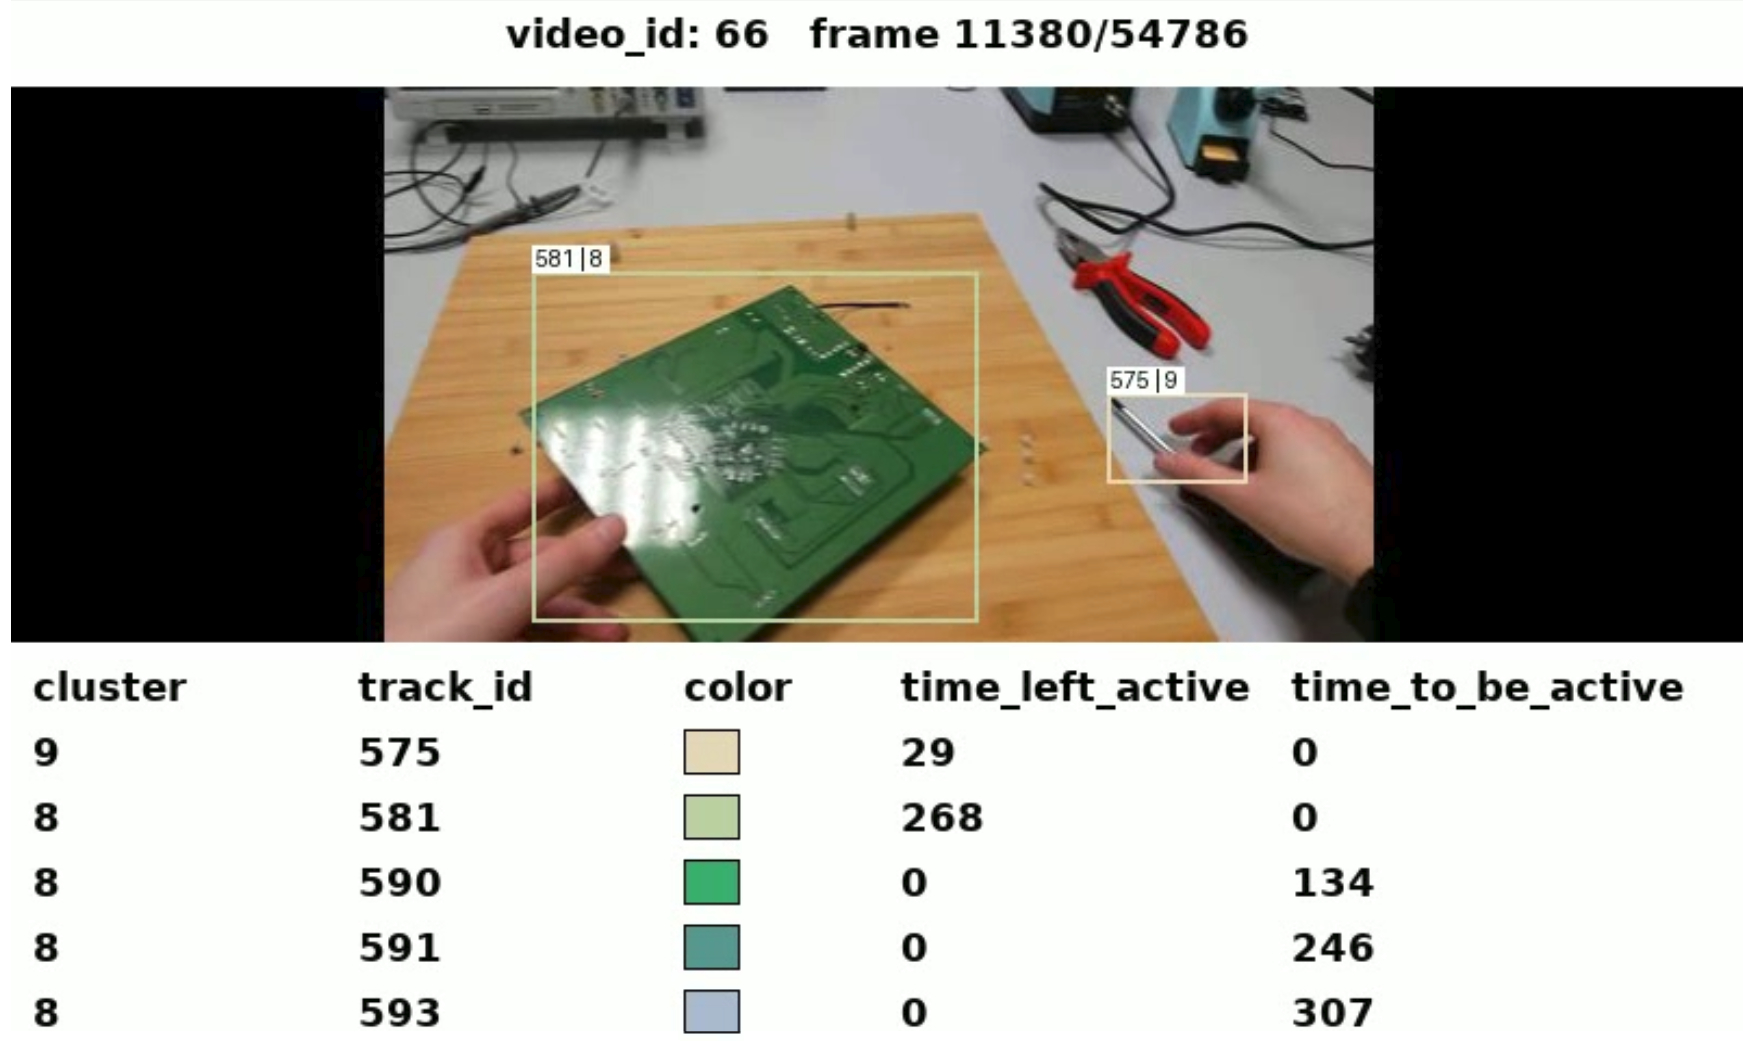
\includegraphics[width=1\linewidth]{Images/amego_video.jpg}
    \caption{visualizzazione degli HOI tracklet del video 66 }
    \label{fig:amego_video}
\end{figure}

Al di sotto del video, una tabella mostra alcune informazioni chiave sugli HOI tracklets visualizzati. In particolare, si riporta il \textbf{Track ID}, il \textbf{Cluster} associato con indicazione dell'ID e del colore univoco, il numero di frame rimanenti in cui il tracklet è ancora attivo (\textit{Time Left Active}) e il numero di frame prima che il tracklet diventi attivo (\textit{Time to be Active}).

\subsection*{Visualizzazione benchmark}
Per avere sempre a disposizione le diverse query, è stato sviluppato uno script che organizza le domande nella seguente struttura:

\begin{verbatim}
<video_id>/
    Q5_00000x/
        VQ/
            <image_patch_1>.jpg
            <image_patch_2>.jpg
            <image_patch_3>.jpg
        Answers/
            <answer_ID>_<class_name>/
                <image_patch_1>.jpg
                <image_patch_2>.jpg
                <image_patch_3>.jpg
\end{verbatim}